\documentclass[12pt]{article}
\usepackage[utf8]{inputenc}
\usepackage[brazil]{babel}
\usepackage{hyphenat}
\usepackage{graphicx}
\usepackage{amsmath}
\graphicspath{{images/}}
\usepackage{float}

% ---- Capa
\title{%
    Modelagem de Sistemas Dinâmicos\\ % \\ pula linha
    \large Trabalho 2}
\author{Erica da Cunha Ferreira }
\date{Novembro 2020}
\begin{document}
\maketitle
\pagenumbering{gobble} 

%-----Sumário
\newpage
\tableofcontents
\newpage
\pagenumbering{gobble} 

%----Pág 1
\cleardoublepage\pagenumbering{arabic}
\section{Introdução}

\quad  Neste trabalho é analisado o motor de corrente contínua (DC) controlado por corrente de armadura com a entrada de tensão $V_a (t)(V)$ e com saídas de posição angular $\theta_m (t)$ e velocidade angular $\omega_m (t)(rad/s)$ representado pela Figura 1.

\begin{figure}[H]
    \centering
    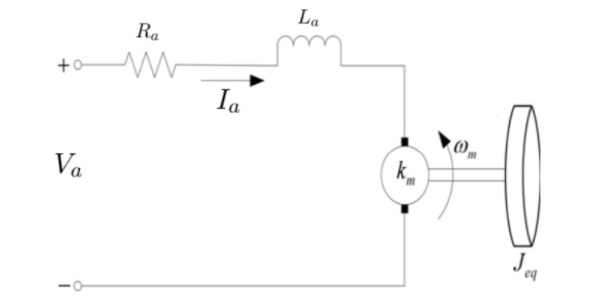
\includegraphics[width = 0.7\textwidth]{Sistema.jpg}
    \caption{Modelo esquemático do motor de corrente continua (DC)}
    \label{fig:mesh1}
\end{figure}

Tendo este sistema as seguintes características fornecidas pelo fabricante:

\begin{itemize}
    \item Resistência da armadura, $R_a$ = 10,6 $\Omega$
    \item Indutância da armadura, $L_a$ = 0,82 $mH$
    \item Momento de Inércia do Rotor do Motor, $J_m = 1,16 10^{-6}$ 
    \item Constantes do Motor, $K_m = K_e =$ 0,0502 $Nm/A$
    \item Tensão Máxima, 15 volts
    \item Massa do disco de inércia, 0,068 $kg$
    \item Raio do disco de inércia, 0,0248 $m$
\end{itemize}

\section{Modelagem Teórica}

\subsection{Representações}

\subsubsection{Diagrama de Blocos}

\quad A partir da análise do circuito e do uso do softwares Matlab e Simulink, pode ser construído o diagrama de blocos da Figura 2, que representa o circuito no domínio da frequência complexa, é importante salientar que o atrito do sistema foi desconsiderado.

\begin{figure}[H] 
    \centering
    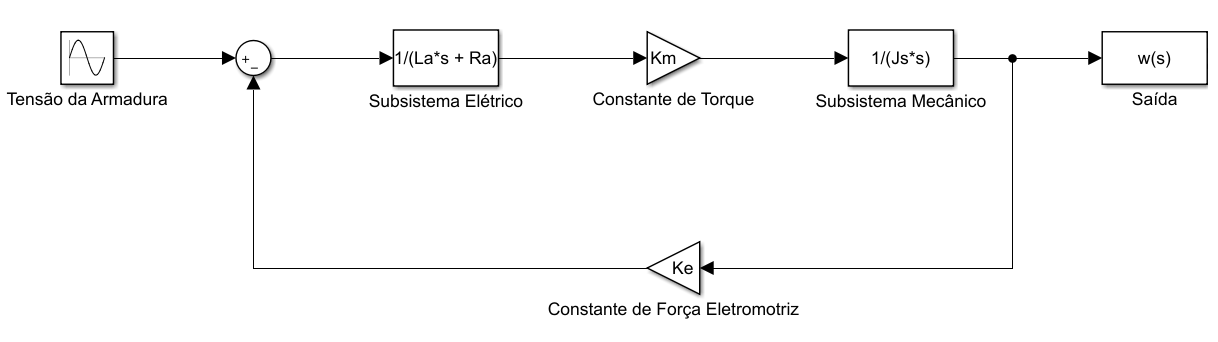
\includegraphics[width=0.9\textwidth]{Blocos.png}
    \caption{Diagrama de Blocos do sistema}
    \label{fig:mesh2}
\end{figure}

\quad Pelo circuito representado pelo diagrama de blocos, as seguintes equações são deduzidas.Considerando que $K_e$ é a constante Eletromotriz, $I_a$ a corrente do motor, $T_m$ torque do motor e $E_m$ a força eletromotriz gerada pelo motor.
\\\par Equações:

\begin{equation}
    V_a (s) = I_a(s) \cdot R_a + s\cdot L_a(s)\cdot I_a (s) + K_e\cdot \omega_m (s)
\end{equation}

\begin{equation}
    J_s\cdot s \cdot \omega_m (s) = K_m \cdot I_a (s)
\end{equation}

\begin{equation}
    T_m = K_m \cdot I_a (s)
\end{equation}

\begin{equation}
    E_m = K_e \cdot \omega_m (s)
\end{equation}

\subsubsection{Função de Transferência}
\quad A partir das informações fornecidas pelo fabricante e do diagrama de blocos, é calculada a função de transferência $G(s)$.

\begin{equation}
    G(s) = \frac{\omega_m (s)}{V_a (s)} = \frac{K_m}{J_s \cdot s \cdot (s \cdot L_a + R_a) + K_m \cdot K_e}
\end{equation}

\subsubsection{Sistema de Espaço de Estados}

\quad O circuito também pode ser representado pelo Sistema de Espaço de Estados, como pode ser visto na equação $(6)$ com $I_a$ representando a corrente.

\begin{equation}
    \dot{x} = 
    \begin{bmatrix} 
        \frac{-R_a}{L_a} & \frac{-K_e}{L_a} \\
        \frac{K_m}{J_s} & 0
    \end{bmatrix}
    \begin{bmatrix}
        I_a\\
        \omega_m
    \end{bmatrix}
    +
    \begin{bmatrix}
        \frac{1}{L_a}\\
        0
    \end{bmatrix}V_a
\end{equation}

\subsection{Momento de Inércia}

\quad A partir dos dados do motor, calcula-se o momento de inércia do disco $I_d$ pela equação $(7)$. Com esse valor, é calculado o momento de inércia do sistema $J_s$, que é dado pela soma do momento de inércia do rotor $J_m$ e do disco $J_d$.

\begin{equation}
    I_d = \frac{mR^2}{2} = 2,091.10^{-5} kg\cdot m^2
\end{equation}

\begin{equation}
    J_s = J_m + I_d = 22,07.10^{-6} kg\cdot m^2
\end{equation}

\subsection{Constantes}

\quad Ao rearranjar a equação $(5)$ e substituir os valores dados pelo fabricante, chegamos à equação:

\begin{equation}
    G(s) = \frac{19,92}{s^2 \cdot (7,1815.10^{-6}) + s\cdot (0,088) + 1} 
\end{equation}

\quad Reajustando os termos, temos:

\begin{equation}
    G(s) = \frac{19,92}{(0,0879\cdot s + 1)(0,0001 \cdot s + 1)}
\end{equation}

\quad Comparando com a equação dada, podemos definir os valores de $K$, a constante de tempo elétrica $\tau_e$, que é determinada considerando que o motor está em estado estacionário e $\tau$.

\begin{equation}
    G(s) = \frac{K}{(\tau s + 1)(\tau_e s + 1)}
\end{equation}

\begin{center}
    $K = 19,92$
\end{center}

\begin{center}
    $\tau = 0,0879$
\end{center}

\begin{center}
    $\tau_e = 0,0001$
\end{center}

Como pode ser visto, devido à ordem do $\tau_e$ quando comparamos com $\tau$, podemos considerar esse valor desprezível. 

\subsection{Valores Máximos}

\subsubsection{Velocidade Máxima}

\quad Ao desconsiderar a pertubação e atrito e ao analisar a equação (1), podemos calcular a velocidade angular máxima $\omega_m(s)$.

\begin{equation}
    V_a(s) = I_a(s)(R_a + L_a(s)\cdot s) + K_e \cdot \omega_m(s)
\end{equation}

\quad Substituindo a equação (3) em função de $I_a(s)$ na equação (12).

\begin{equation}
V_a (s) = \frac{J_s(s) \cdot s \cdot \omega_m(s)}{K_m}\cdot R_a(s) + K_e \cdot \omega_m    
\end{equation}

\quad Utilizando o Teorema do Valor Final (14), o $s$ tende a 0, resultando na equação (15).

\begin{equation}
    \lim_{t \to \infty} f(t) = \lim_{s \to 0} sF(s)
\end{equation}

\begin{equation}
    \omega_{max} (s) = \frac{V_a(s)}{K_e} = \frac{15}{0,0502} = 298,804 \frac{v.A}{Nm}
\end{equation}

\subsubsection{Corrente e Torque Máximos}

\quad Ao analisar o sistema em regime estacionário e nas condições citadas anteriormente, podemos dizer que a Força eletromotriz $E_m$ gerada pelo motor é igual a 0, uma vez que não há movimento. Por causa disso, a equação (1) pode ser reescrita. Além disso, é possível afirmar $I_as = 0$, uma vez que no regime estacionário, não há variação de corrente. Logo temos a expressão (16). 

\begin{equation}
    R_a I_{max}(s) = V_a(s)
\end{equation}

\quad Substituindo na equação (16) os valores dados pelo fabricante, temos:

\begin{equation}
    I_{max} = \frac{V_a(s)}{R_a} = \frac{15}{10.6} = 1.415 A
\end{equation}

\quad Ao analisar a equação (3) e colocar os os valores do fabricante, temos:

\begin{equation}
    T_{max} = K_m \cdot I_{max}(s) = 0.0502 \cdot 1.415 = 0.071 Nm
\end{equation}

\section{Identificação Experimental}

\subsection{Motor Parado Forçadamente}

\quad Os dados das Tabelas (1) e (2) foram obtidos experimentalmente pelo kit QET da Quanser. 

\begin{table}[H]
\centering
\begin{tabular}{c c} 
 \hline
 $V_a(V)$ & $I_a(A)$ \\ 
 \hline
 1.0 & 0.076 \\ 
 2.0 & 0.150 \\
 3.0 & 0.225 \\
 4.0 & 0.305\\
 4.9 & 0.425\\
 5.9 & 0.474\\
 6.9 & 0.550\\
 7.9 & 0.620\\
 8.9 & 0.720\\
 9.9 & 0.800\\
 \hline
\end{tabular}
\caption{Medição realizada com o eixo do motor forçadamente parado}
\label{table:data1}
\end{table}

\quad Ao considerar o eixo motor parado, a equação (1) se transforma na equação abaixo:

\begin{equation}
    R_a = \frac{V_a}{I_a}
\end{equation}

\quad Então podemos calcular a resistência da armadura $R_a$ estatisticamente  a partir do coeficiente angular do gráfico abaixo:

\begin{figure}[H] %h é para here - aqui
    \centering
    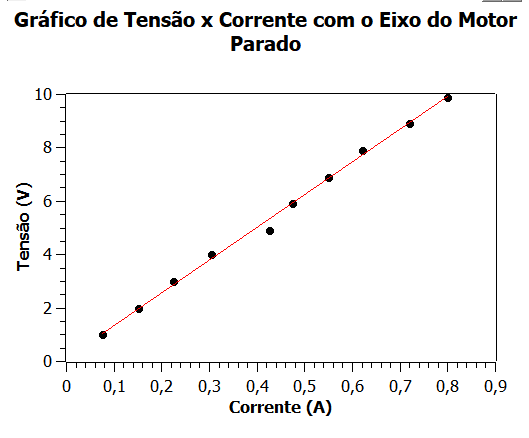
\includegraphics[width = 0.7\textwidth]{GRÁFICO 01.png}
    \caption{Gráfico do eixo do motor parado forçadamente}
    \label{fig:mesh3}
\end{figure}

\begin{equation}
    R_a = \frac{V_a}{I_a} = 12,2 \Omega
\end{equation}

\subsection{Motor Sem Carga}
\begin{table}[H]
\centering
\begin{tabular}{c c c} 
 \hline
 $V_a(V)$ & $\omega_m(rad/s)$ & $i_a(mA)$ \\ 
 \hline
 1.0 & 12 & 1 \\ 
 2.0 & 29 & 1 \\
 3.0 & 49 & 1 \\
 4.0 & 70 & 1\\
 4.9 & 89 & 1\\
 5.9 & 105 & 1\\
 6.9 & 127 & 2\\
 7.9 & 148 & 2\\
 8.9 & 168 & 2\\
 9.9 & 185 & 3\\
 \hline
\end{tabular}
\caption{Medição realizada com o motor sem carga}
\label{table:data2}
\end{table}

\quad A constante de torque do motor $K_m$ também pode ser calculada estatisticamente a partir do coeficiente do gráfico abaixo, que por sua vez são os valores fornecidos pela a Tabela (2) plotados.

\begin{figure}[H] %h é para here - aqui
    \centering
    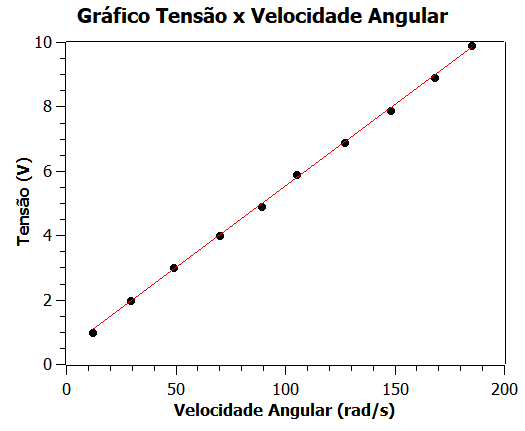
\includegraphics[width = 0.7\textwidth]{GRÁFICO 02.png}
    \caption{Gráfico do motor sem carga}
    \label{fig:mesh4}
\end{figure}

\begin{equation}
    K_m = \frac{V_a}{\omega_m} = 0,0506 Nm/A
\end{equation}

\quad Também podemos calcular a função de transferência $\hat{G}(s)$ e então achar o $\hat{\tau}$ e o $\hat{K}$, que são os valores achados experimentalmente.

\begin{equation}
    \hat{G}(s) = \frac{19,76}{(0,1051 s + 1)(0,0001 s + 1)}
\end{equation}

\begin{equation}
    \hat{G}(s) = \frac{19,76}{(0,1051s + 1)}
\end{equation}

\begin{center}
    $\hat{\tau} = 0,1051$\\
\end{center}

\begin{center}
    $ \hat{K} = 19,76$
\end{center}

\section{Validação dos Modelos}

\subsection{Resposta ao Degrau}

\quad Para esta simulação, foi aplicado um gerador de pulsos constantes de amplitude de 5 volts no motor e a resposta ao degrau. Temos então o seguinte gráfico plotado pelo Simulink.

\begin{figure}[H] %h é para here - aqui
    \centering
    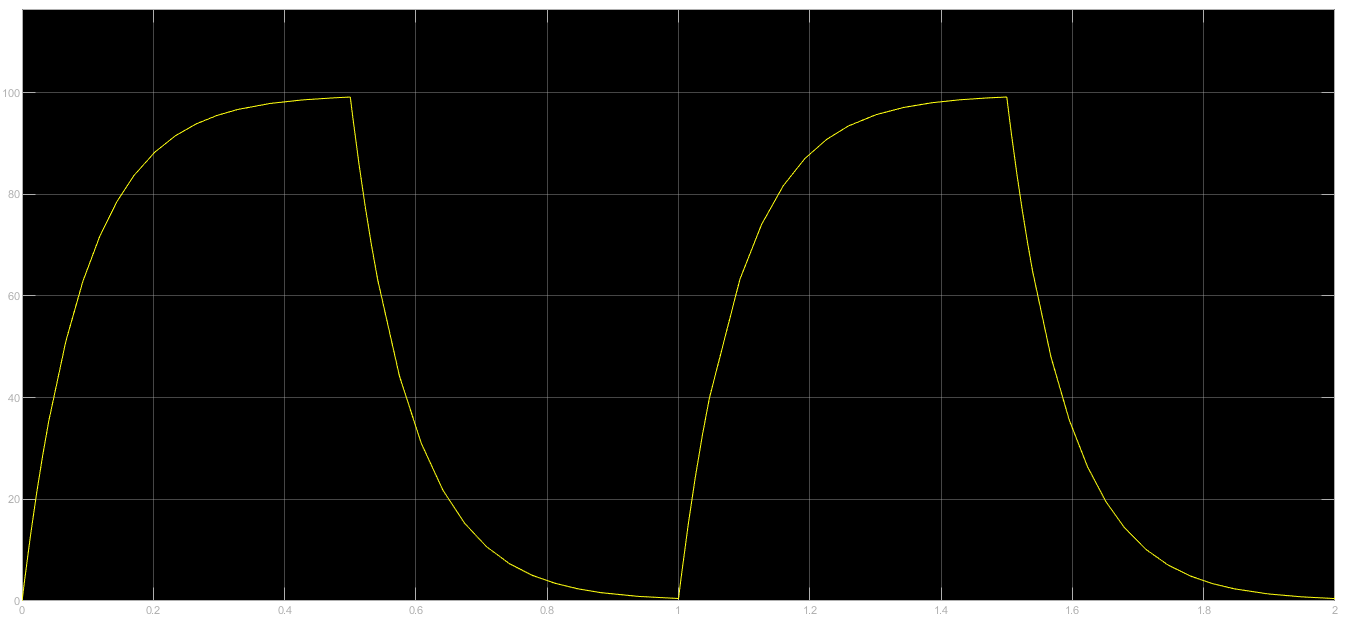
\includegraphics[width = 1\textwidth]{Imagem_matlab.png}
    \caption{Gráfico}
    \label{fig:mesh5}
\end{figure}

\quad A partir da Figura (5) podemos quantificar o ganho real $K_r$, que é calculado pela razão entre a velocidade máxima $\omega_{max}$ e a tensão máxima $V_{max}$. 

\begin{equation}
    K_r = \frac{\omega_{max}}{V_{max}} = 19,828
\end{equation}

\quad A constante de tempo real $\tau$ por sua vez, é calculado pela quantidade de tempo entre quando o sistema está com a velocidade 0 e quando ele atinge $63\%$ da velocidade máxima. 

\begin{center}
    $\tau_r = 0,091$
\end{center}

\subsection{Comparação}

\quad Agora que temos os valores teóricos, experimentais e reais, podemos compará-los.

\subsubsection{Diferença entre real e teórico}

\quad Calcule-se o erro percentual pela seguinte fórmula.

\begin{equation}
     \epsilon (\%) = |Valor_{real} - Valor_{medido}|\cdot 100
\end{equation}

\quad Ao substituir na equação (23) os valores encontrados pela simulação no Simulink e os encontrados teoricamente, temos os seguintes erros percentuais.

\begin{center}
      $\epsilon_{\tau}(\%)  = 3,4 \%$
\end{center}

\begin{center}
      $\epsilon_{K}(\%) = 0,464\%$
\end{center}

\subsubsection{Diferença entre real e experimental}

\quad Ao substituir na equação (23) os valores encontrados pela simulação no Simulink e os encontrados estatisticamente pelos os valores experimentais dados pelas tabelas, temos os seguintes erros percentuais.

\begin{center}
     $\epsilon_{\tau}(\%) = 15,5 \%$
\end{center}

\begin{center}
     $\epsilon_{K}(\%)= 0,343\%$
\end{center}
\section{Conclusão}

\quad Ambos os modelos obtiveram erros percentuais baixos, entretanto, ao compararmos os dois modelos, teórico e experimental, pode-se perceber que o teórico tem um erro menor. Isto se deve ao fato de que os valores experimentais serem retirados manualmente, o que abre a possibilidade para os mais variados erros acontecerem, como o erro da pessoa que os mediu e erros instrumentais, como o do software. Já que alguns valores tem uma ordem pequena, vide o $\tau$, um erro de algumas casas decimais pode interferir significativamente.
\par Conclui-se, então, que o modelo teórico tem uma maior compatibilidade com o modelo real, uma vez que os erros instrumentais interferem na acurácia do modelo experimental.
\end{document}

